% \documentclass[review]{elsarticle}
\documentclass[final,3p,times,onecolumn,sort&compress]{elsarticle}

\usepackage{lineno,hyperref}
\usepackage{listings}
\modulolinenumbers[2]

\usepackage{array}
\newenvironment{conditions}
  {\par\vspace{\abovedisplayskip}\noindent\begin{tabular}{>{$}l<{$} @{${}={}$} l}}
  {\end{tabular}\par\vspace{\belowdisplayskip}}
\newcolumntype{R}{>{\raggedleft\arraybackslash}m{2cm}}


\lstset{language=Python,
    basicstyle=\footnotesize\ttfamily,
    % commentstyle=\ttfamily\itshape\color{gray},
    stringstyle=\ttfamily,
    showstringspaces=false,
    breaklines=true,
    frameround=ffff,
    frame=single,
    % rulecolor=\color{black},
    tabsize=1,
    % keywordstyle=\color{red}\bfseries,
    columns=fullflexible,
    morekeywords={public, class}
    morecomment=[s]{"""}{"""},
}

\journal{ }

%% Elsevier bibliography styles
%% APA style
\bibliographystyle{model5-names}\biboptions{authoryear}

%%%%%%%%%%%%%%%%%%%%%%%

\begin{document}

\begin{frontmatter}

\title{A global measure of inequality in the built environment: Evaluating grocery store access for planning policy and intervention}

% \author[]{T M Logan\corref{mycorrespondingauthor}}
% \ead{tom.logan@canterbury.ac.nz}
% \author[]{M J Anderson}

% \address{Civil and Natural Resources Engineering, University of Canterbury, New Zealand}

\begin{abstract}
The built environment has institutionalized many of the inequities prevalent in our society.
<something's missing here>
While inequity and inequality are often evaluated for income, there are many other goods, services, and also undesirable quantities (such as exposure to environmental harm) that are distributed throughout our communities.
To understand and address inequity in how these quantities are distributed, we need to measure and identify inequality.
To go beyond equality, we need the ability to evaluate inequality between subgroups within our communities.
However, existing approaches to evaluating the equality of distributions are insufficient or, in the case of undesirable quantities, mathematically unsuitable.
Recently, in the risk science literature, a quantitative measure for the performance and inequality of a distribution was presented for evaluating the equality of health risk.
In this paper, we demonstrate how this measure (which uses the \textit{equally-distributed equivalent}: EDE) and associated index could be used in an urban planning and hazard contexts to support decision making to foster equity in the built environment.
We use examples of food access in cities across the USA and post-hazard recovery as illustrations.
\end{abstract}

\begin{keyword}
Urban planning $|$ Equity $|$ Environmental justice 

\end{keyword}

\end{frontmatter}

\linenumbers

\section{Introduction}
As our cities undergo the major and rapid changes brought on by climate change, population growth, the urban renaissance, and neoliberalism, there is a major risk of deepening inequalities worldwide \citep{nijman}.
These changes include how environmental burdens are distributed across our society, from exposure to natural hazards sea level rise, to vulnerability to chronic diseases and gentrification. 
The changes will also include attempts to ameliorate these issues and provide urban amenities, but these resources also must be distributed fairly so everyone has the same opportunities to prosper.
To ensure this fairness in distribution, planners, policy makers, designers, and engineers need the ability to evaluate scenarios in a substantive manner.

Fairness, and what it constitutes, is characterized by the concepts of equality, equity, and environmental justice \citep{talen, low, rigolon, lopez}.
In this paper, we consider equality to be homogeneity across the recipients of a resource, whereas equity is the attempt to deliver justice \citep{rumley}.
For example, \cite{rumley} provided the anecdote that giving two children each an apple achieves equality; however, if one child had not eaten in three days, then the goal of equity is not met. 

Urban form and the built environment has a significant influence on equity within our communities.
How we design our communities and react to hazards, drives how burdens and resources are distributed between our people \citep{wilson}.
These burdens include exposure to natural hazards \citep{}, chronic diseases \citep{}, hours spent commuting \citep{}, and air pollution \cite{Maguire2011-fi, Sheriff2020-ge}.
Resources, many of which ameliorate some of these burdens, include trees \citep{nesbit} and amenities like supermarkets, schools, health care, green space.
For example, access to healthy food improves peoples' diets, which improves their health \citep{garcia, kolak}.
Whereas green space mitigates flooding, heat, erosion, and air pollution, while providing opportunities for recreation, improved mental health, and the forging of social capital \cite{Williams2020-greenspace}.

However, it is not enough that these be spread equally through a community.
Firstly, some degree of geographic inequality is inevitable \citep{dadashpoor}, but primarily, some groups simply need more of some resources than others.
For example, youth need access to schools, while older people need higher access to health care \citep{syed}.
Older people, at risk of social isolation, also need higher access to green space where they can build their social capital \citep{frumkin}
Additionally, groups with increasing rates of obesity (women, racial-minorities, and low-income communities \citep{day}) need improved access to healthy food outlets \cite{garcia, Kolak2018-az} and environments that promote physical activity \citep{krenichyn}.
Finally, minority groups who were subject to discriminatory housing policies over 50 years ago are still experiencing the consequences with high rates of unemployment and chronic disease \citep{white-redling}.
That is to say, equality alone is insufficient.
Instead, environmental justice --- the notion that everyone has the right to a healthy environment \citep{lopez} --- is achieved through equity in distributional, procedural, and interactional justices \cite{low}.
Where we place resources and guide residential development dictates distributional justice.
How we create spaces influences interactional justice, as approaches such as mixed-use design encourage a diversity of users and enables people to interact safely \citep{jacobs}.
And whether communities are empowered and engaged during the decision-making process has an influence on procedural justice \citep{low, rigolon}.

The benefits of equity also includes enhanced community sustainability and resilience \cite{Dempsey2011-og, cutter, Logan2020-vj}.
This is because equity fosters community trust and cohesion; attributes that the ongoing pandemic is highlighting the benefits or failings of, worldwide.

Analyzing equity begins with an analysis of equality, that must then be coupled with an evaluation of need or social justice \cite{talen-anselin1998}.
Therefore, to measure equity, we must be able to measure equality and repeat it for various subgroups.
However, existing measures of inequality have had major limitations that have restricted their utility in urban planning. 
A recently proposed measure of equality --- the Kolm-Pollak method --- has removed those limitations \citep{Sheriff2020-ge} and thus, we believe, enables numerous opportunities for planners.
The objective of this paper is to demonstrate how this Kolm-Pollak approach can be used in a planning context to provide a substantive measure of evaluating interventions based on both the overall utility and effect on equity.

\section{Measuring equality}
\cite{Pacione1989-ui} uses CV to examine the effect of school closures


Urban form and the built environment have a significant influence on equity within our communities.
Equity in society has a major impact on community trust and cohesion, and, in turn, community sustainability and resilience.
One factor influencing this community sustainability and resilience that planners can influence is distributional equity (the equity in proximity) of urban amenities.
Access to essential services is essential for communities to thrive \cite{Dempsey2011-og, United_Nations_Educational_Scientific_and_Cultural_Organization2018-sf, Winter1997-kc} and disparities in this access limit the potential of those affected and, as a result, the wider community.
For example, systematic differences in urban form can affect people's access to healthy food and that can perpetuate health disparities \citep{Kolak2018-az}.
Also, access to services is associated with improved resilience \cite{Frazier2013-ct}.
Access is an important consideration both in normal times as well as following disasters, which can often exacerbate existing inequalities and access-deserts.
The equitable distribution of many amenities has been studied, including green space \citep{Rigolon2018-jl}, urban trees \citep{Schwarz2015-fs}, medical facilities \citep{Apparicio2008-nq}, food \citep{Walker2010-ch}, playgrounds \citep{Talen1998-mk}, service stations \citep{Logan2020-vj}, education \citep{Pacione1989-ui}, cultural facilities \citep{United_Nations_Educational_Scientific_and_Cultural_Organization2018-sf}, and many others. 
Without access to these and other essential services, communities can collapse, which occurred in the relocated communities following the L'Aquila earthquake in Italy \citep{Contreras2017-yq}.
Additionally, the distribution of unwanted facilities and environmental injustices is also particularly important to understand and quantify \citep{Talen1998-fl}.
In light of the on-going pandemic, access is particularly pertinent as people without private vehicles are either unable to access critical services or are disproportionately exposed through long commutes on public transit.
As accessible, equitable urban form is important for both sustainability and resilience, it is only increasing in importance. 
Measuring and identifying inequity can motivate decision-makers to incentivize development to ameliorate and address these inequities \citep{Kolak2018-az}.




The ability to assess inequity is, therefore, essential for planners \citep{Talen1998-fl}.
Approaches to doing so include maps (e.g., \cite{Talen1998-fl}), plots of the statistical distribution \citep{Logan2019-fr}, and statistics such as the Gini coefficient or percentage of residents within some threshold. 
Map-based visualization approaches are irreplaceable as they identify the specific regions lacking in or over exposed to the quantity in question. 
The maps are also essential for communication with decision-makers and residents so they can appreciate the geographic arrangement of resources and visualize the unequal distribution \citep{Talen1998-fl}.
As a complement to the maps, a quantitative measure is necessary to support analysis such as ranking of interventions, ranking of cities for allocating assistance, or for optimization in a manner that visualizations are unable to support (e.g., Figure \ref{fig:the_challenge}).
One option is to use summary statistics such as the mean or the percentage of residents within some threshold.
However, these measures can introduce substantial error (discussed in \cite{Kolak2018-az} and \cite{Logan2019-fr}) and do not reflect the inequality or penalize a distribution for it (e.g., Figure \ref{fig:problem_with_existing}).

\begin{figure}[h]
    \centering
    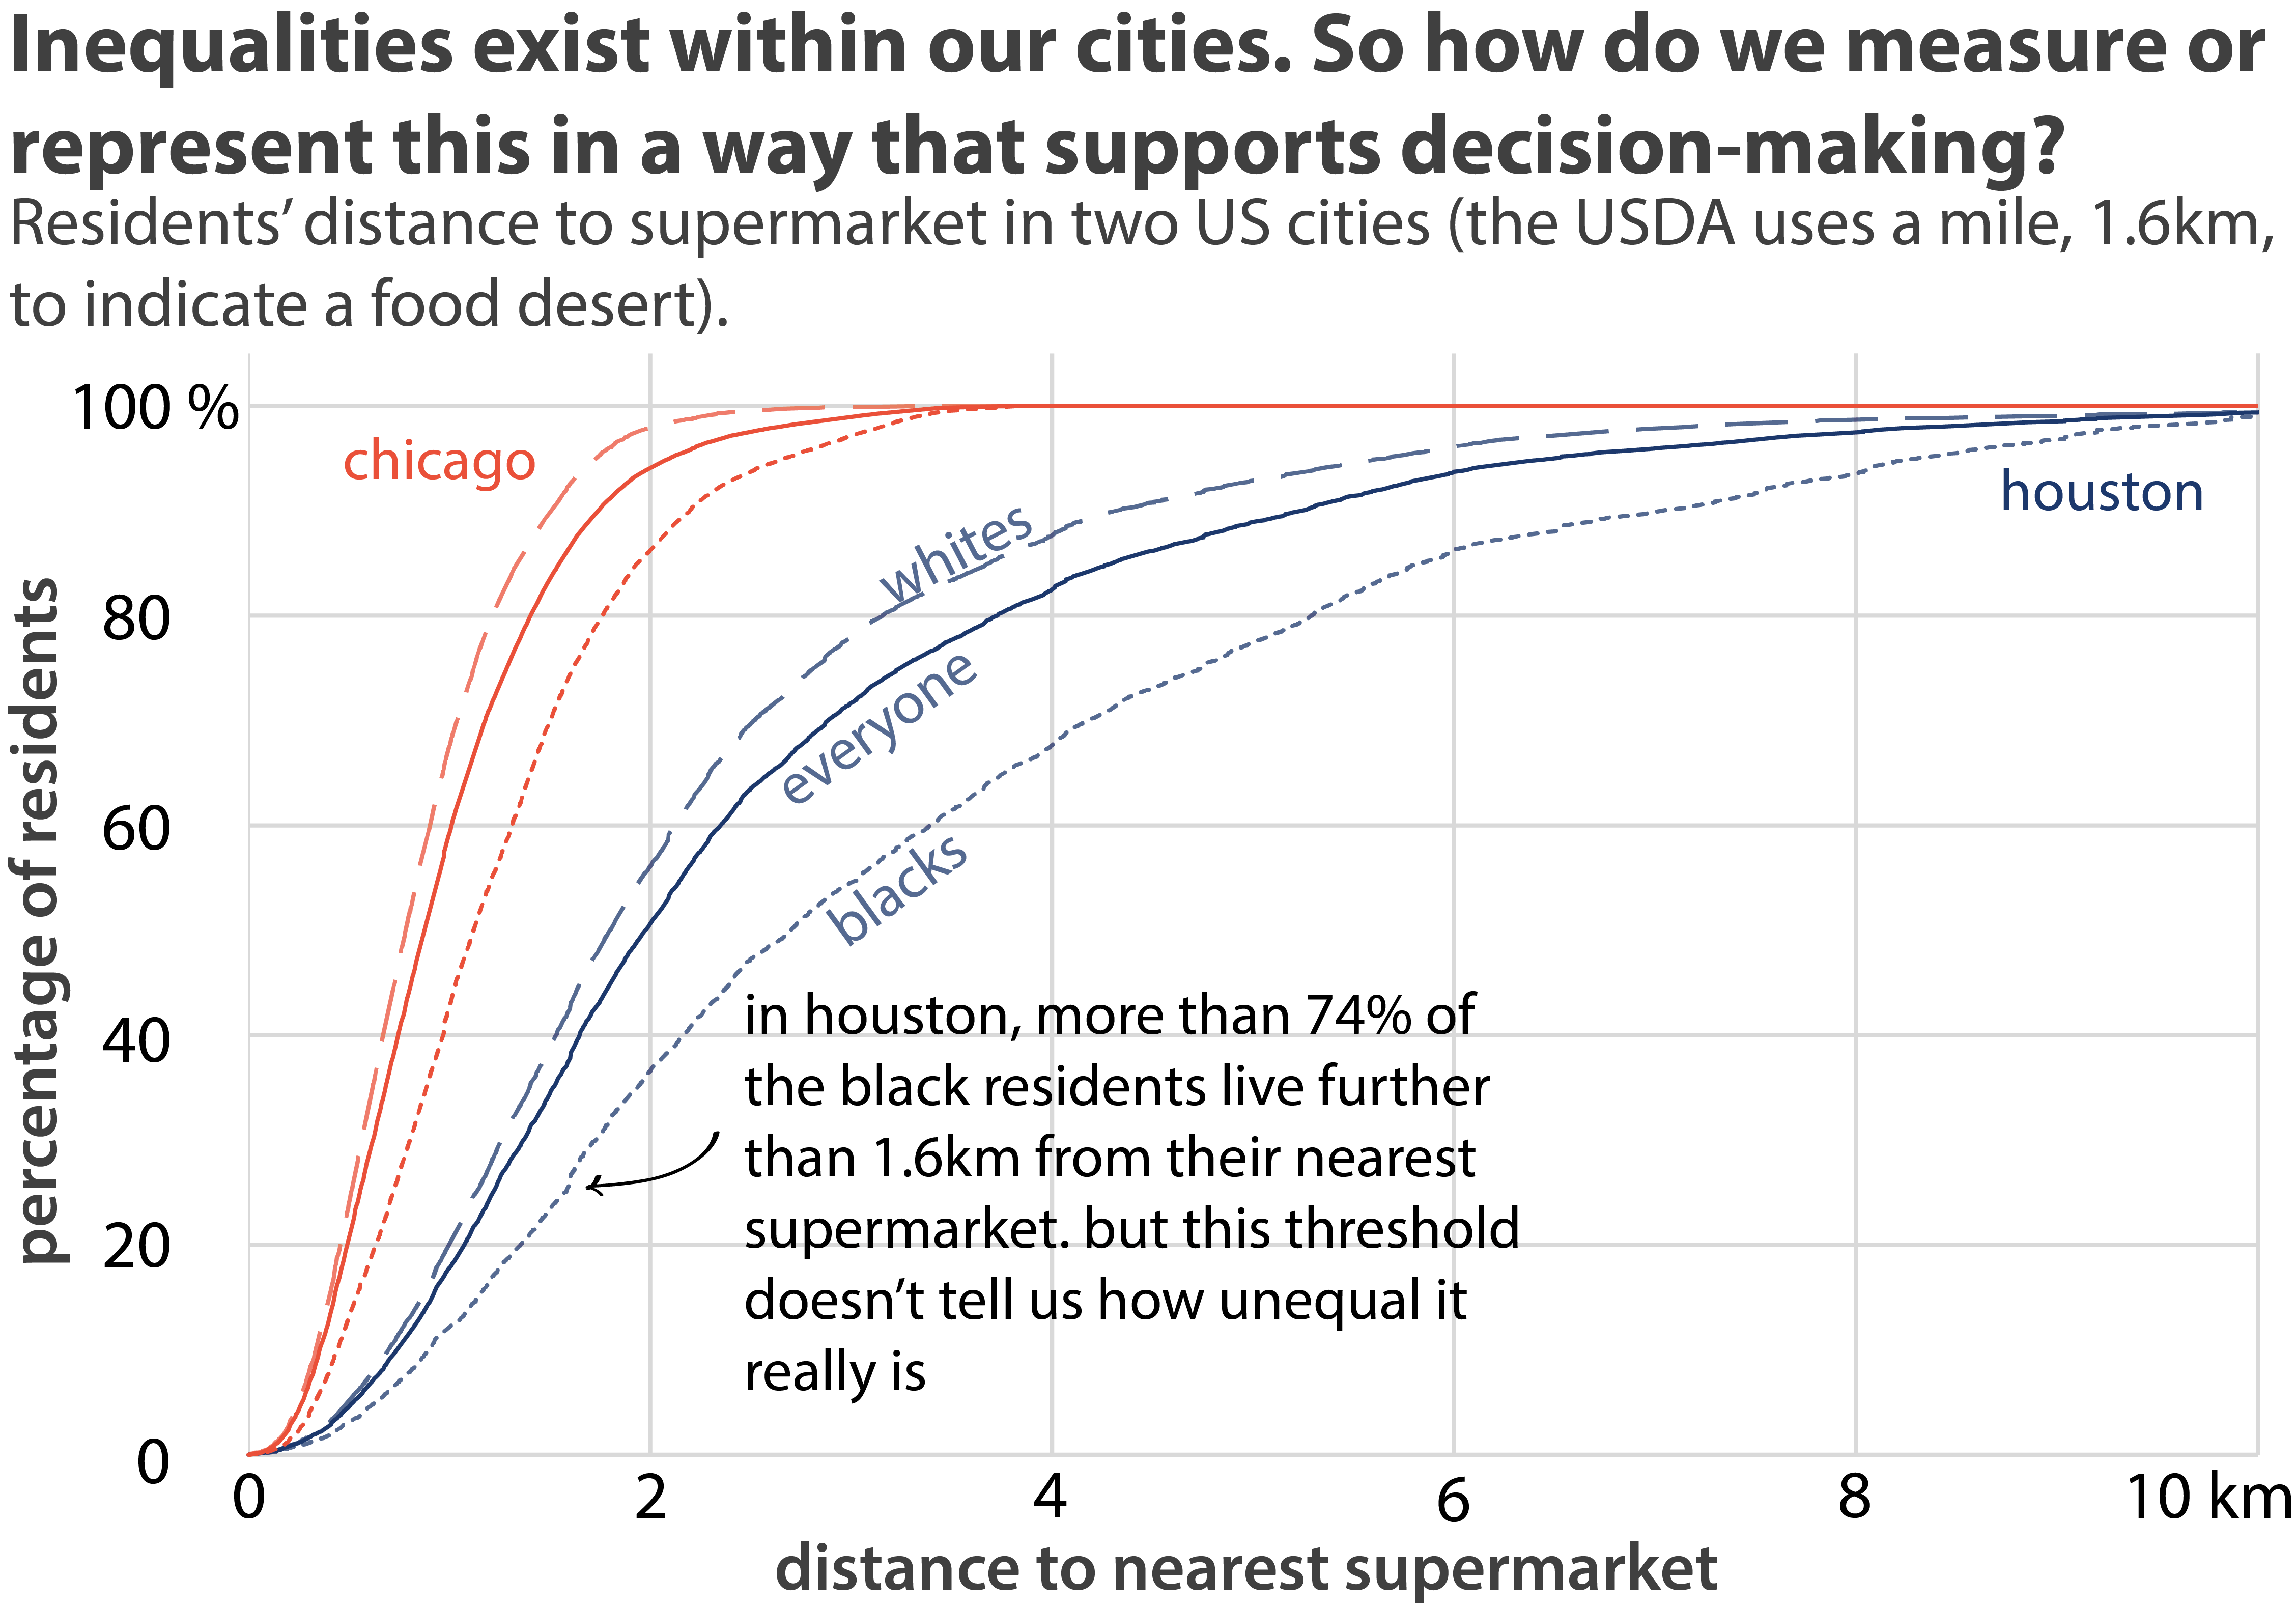
\includegraphics[width=0.5\linewidth]{report/fig/fig1.png}
    \caption{
    How should we quantitatively represent how a quantity is distributed through a community? This is an example with supermarket proximity in Chicago and Houston.
    }
    \label{fig:the_challenge}
\end{figure}

\begin{figure}[h]
    \centering
    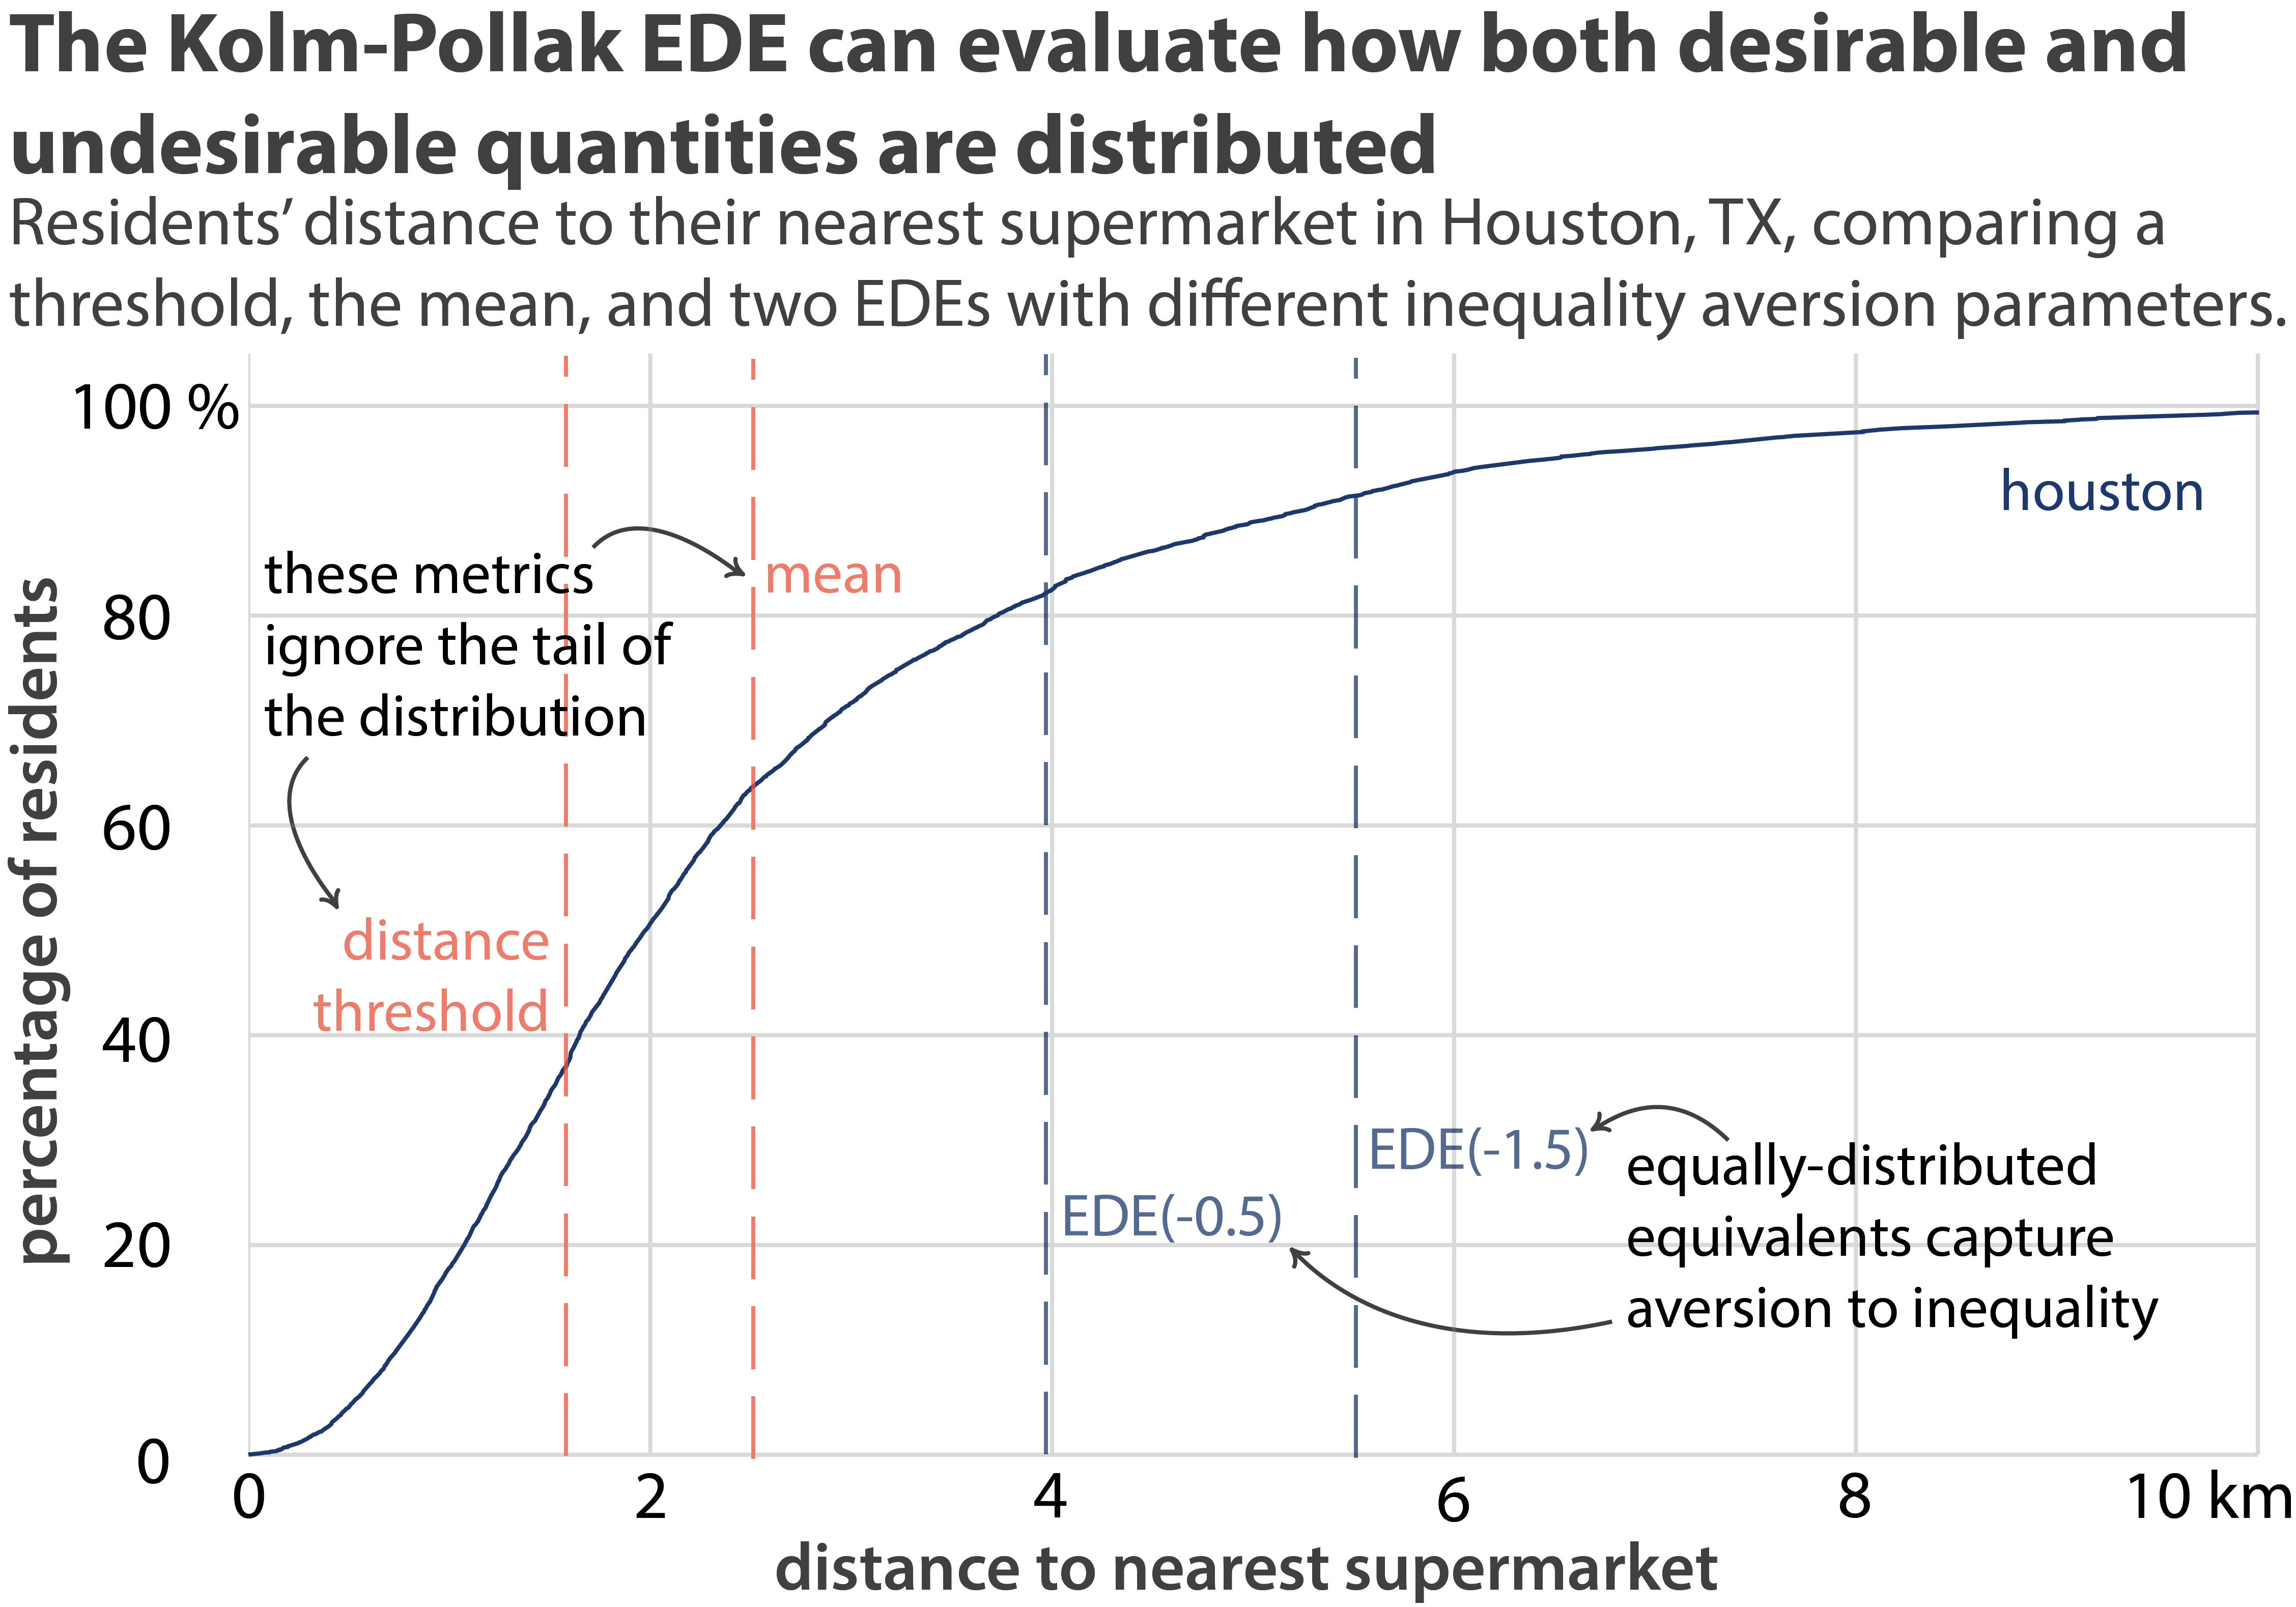
\includegraphics[width=0.5\linewidth]{report/fig/fig1b.png}
    \caption{
    Traditional measures for representing distributions fail to reflect how poorly-off some residents are. For example, the threshold is completely indifferent of the distribution of people beyond that threshold. 
    The EDE's are an option that accounts for the tail of the distribution.
    }
    \label{fig:problem_with_existing}
\end{figure}

Existing measures of equality include the Gini Coefficient, the Atkinson Index, and the coefficient of variation.
Of these, the Gini Coefficient is the most commonly used \citep{Whitehead2019-tf, Maguire2011-fi}.
An advantage of the Gini Coefficient is its simplicity, as it represents how a distribution differs from perfect equality.
The coefficient of variation is also mathematically straightforward and is a commonly used measure in statistics.
However, there are a number of disadvantages (outlined in \cite{Maguire2011-fi, Atkinson1970-mr, Adger1997-tu}) that make them both unsuitable or unsatisfactory for many applications.
The most important disadvantage for these measures is how they prioritize wealth transfer.
Essentially, neither prioritizes improving the situation of the worst-off individuals.
As both measures are `positive,' meaning they require no value judgement, they simply report the dispersion (spread) of a distribution and are indifferent to whether that inequality is at the top or bottom of the distribution.
Another disadvantage is that comparing distributions based on their Gini coefficient or coefficient of variation is relatively uninformative.
The main reason for this is that they are relative inequality indices; that is, the absolute value does not matter.
This is useful if you want to compare the inequality between distributions without considering their absolute value; 
for example, this enables the comparison of wealth inequality between countries with different total wealth.
However, in situations of interest to planners and city engineers, the absolute value of a distribution matters and it is plausible that a less equal distribution may be the more desirable in some instances.
For example, in a hazards context, a situation in which everyone is equally majorly affected by an event is likely less desirable than one where some residents are not impacted while the others are minorly effected, even though this latter case is less equal.

To address these limitations, \cite{Atkinson1970-mr} proposed using a social welfare function and introduced the equally-distributed equivalent (EDE) to represent a distribution in a manner that reflects its inequality. 
The EDE represents the value which would, if everyone had that same value, provide the same level of welfare as the existing distribution.
An EDE is analogous to the risk premium or certainty equivalent from decision science and is, in practice, an alternative summary statistic for a distribution that captures both the location (c.f. the mean or median) and the dispersion (c.f. the variance) of a distribution.  
Unlike other summary statistics, however, the EDE is based on a subjective parameter that represents aversion to inequality and is how welfare is determined.
The use of this parameter shifts the value judgment regarding the importance of inequality from being implicit, as it is for the Gini coefficient and coefficient of variation, to being explicit and user defined.
While some users are uncomfortable with the subjectivity of a user-defined parameter, this is a somewhat false claim, given that the act of choosing an alternative measure is to also make a value judgement regarding the user's aversion to inequality. 
Instead, using a measure with an explicit aversion to inequality enables us to evaluate the sensitivity of rankings of alternative interventions to that aversion.
Besides, as \cite{Atkinson1970-mr} points out, any evaluation of inequality involves judgements relating to social welfare - a normative approach enables us to explore the affect of these judgements.

While the Atkinson index has proven useful for evaluating the inequality of income, it is unsuitable for distributions of undesirable quantities \citep{Cox2012-lg, Sheriff2020-ge, Maguire2011-fi} --- a crucial question of planners.
Simply inverting an undesirable distribution to evaluate the equality of the complement (e.g., using $\frac{1}{x}$ instead of x) does not address this problem because the order of preference when comparing distributions can change between the undesirable quantity and its complementary good \citep{Sheriff2020-ge}.
This issues with the Atkinson index was recently addressed through adjustments to the Kolm-Pollak index \citep{Sheriff2020-ge}.

The Kolm-Pollak measure of inequality is similar, although mathematically distinct from the Atkinson measure.
It also uses an inequality aversion parameter and produces an EDE.
However, it differs from the Atkinson in that i) it has been constructed to evaluate the distribution of undesirable quantities; and ii) outputs an absolute inequality index.
Additionally, both the Atkinson and Kolm-Pollak measures is the option of subgroup decomposition. 
Subgroup decomposition enables us to evaluate inequity in addition to inequality, and confront environment justice issues. 
Without considering the socioeconomic and racial/ethnic status means we are unlikely able to address the underlying inequalities in the existing social structure \citep{Talen1998-fl}.

Ultimately, EDE's enable us to \citep{Sheriff2020-ge}: 
\begin{itemize}
    \item compare how a range of interventions impact the distribution
    \item evaluate how different demographic groups are affected by each intervention
    \item determine, for a given demographic group, which intervention is preferred
    \item identify which groups benefit the most from an intervention
    \item understand how equality changes over time (for example, following a hazard).
\end{itemize}
The EDE can also be used as a descriptive statistic that could be used in other analysis, such as regression, instead of other descriptive statistics that do not include inequality.
For example, \cite{Rigolon2018-jl} uses a regression across 100 US cities to determine if access to green space is associated with socioeconomic factors of those cities.
While they use the ParkScore rating, which is based on \% of people within a ten-minute walk from a park, they could also use an EDE to capture both the average state of access, but also the inequality.

A measure of a distribution and its inequality presents a suite of opportunities for those working with the built environment.
It enables us to understand how changes in urban form may differentially impact the community.
For example, we can evaluate interventions such as the closure of a high school, the opening of a supermarket, the implementation of a hazard-zoning policy, or the impact from and recovery following a disaster.
It also enables us to compare and rank alternative interventions while considering inequality.
This means that consideration of inequality can be included in decision making.

While \cite{Sheriff2020-ge} caveat that EDEs have limitations, none are surprising.
The EDE describes the distribution of the quantity in question.
The inequality index, therefore, describes the inequality in that quantity's distribution.
\cite{Cox2012-lg} criticized the use of inequality indices for health risks as being ``neither logically coherent nor necessarily ethically desirable.''
One foundation of this argument was the point that inequality indices only measure a single quantity (rather than multiple criteria). 
He argued that, for example, some people may choose higher exposure to air pollution and would ameliorate that with lower property prices, allegedly balancing the inequality. 
This argument appears to ignore the history of social, racial, and environmental injustices and assumes that everyone has the privilege of choice.
Nevertheless, although the justification is unsound, the point remains that equality indices are constructed with respect to a single quantity.
However, there is no reason that equality indices cannot be constructed for multiple attributes and characteristics (e.g., one for health risk, one for property value, etc.) and then analyzed or regressed so to evaluate these wider inequalities.

To demonstrate the utility of the Kolm-Pollak approach for measuring the performance of and equality of a distribution, we use three illustrative examples.
The first is access to grocery stores in ten cities in the USA.
Food deserts present a significant issue for inequity \citep{Kolak2018-az, Walker2010-ch}.
While definitions of food deserts vary \citep{Walker2010-ch}, proximity to the nearest grocery store is a common factor in these measures.
For example, the USA's Department of Agriculture defines a food desert as an area that is further than a mile (1.6km) from the nearest large grocery store.
In this study, we evaluate the proximity to nearest grocery store in ten US cities and evaluate the disparities between racial and ethnic groups.
While our study is not a comprehensive review of food deserts --- as we do not do the rigorously validate the provision and acceptability of each supermarket, as outlined in \cite{Kolak2018-az} --- this study nonetheless investigates the equity of grocery store access throughout these cities and enables the demonstration of assessing distributions of quantities within the built environment.
We use this case study to also explore the sensitivity of our results to the aversion parameter.
The example demonstrates how the Kolm-Pollak can be used to compare and rank different distributions and investigate how demographic groups are affected by those distributions.

With our second example, we demonstrate how the change in a distribution over time can be examined.
This is the case of how grocery store access for a community is impacted by a disaster: how resilient the community's food access is, including the robustness and speed of recovery, and the equity of both the existing form and the recovery process. Specifically this is a case study using the city of Wilmington, North Carolina, as it was impacted by Hurricane Florence in 2018.
We can use the Kolm-Pollak to measure the performance and inequality of supermarket access and how that changed due to the hurricane and subsequent recovery.

Finally, to demonstrate that the approach has opportunities in the built environment beyond access, we evaluate the impact of Hurricane Matthew on electricity provision across a number of USA states.
We compare unnamed states and power companies regarding both how their network was impacted and on the restoration times.

As a complement to the paper, we provide publicly available Python functions for calculating inequality metrics for a distribution. 
This code is available in \ref{appendix:code} and at [GitHub address redacted for review].

\section{Methods and Data}
\subsection{Measures of distributions}
\subsubsection{Kolm-Pollak}
In this paper we demonstrate how the Kolm-Pollak EDE and inequality index can be used in the built environment to measure the absolute performance and inequality of some distribution.
For comparison, we also apply several of the existing alternatives. 
However, the Kolm-Pollak is the only mathematically suitable measure (as described earlier) because: i) like the Atkinson EDE and in contrast to the Gini coefficient, it measures absolute performance; and ii) it can be used, unlike the Atkinson, to assess distributions of both desirable and undesirable quantities.

The Kolm-Pollak represents the absolute performance of a distribution using an equally-distributed equivalent (EDE).
This is the value that states the position within the distribution which make an individual indifferent between the scenario where everyone receives the value of the EDE and the existing unequal distribution.
The EDE is calculated for a distribution of $X$ using \citep{Sheriff2020-ge}
\begin{equation}
    y_{EDE} = -\frac{1}{\kappa} \ln \left[ \frac{1}{N} \sum_{i=1}^{N} e ^ {-\kappa x_i} \right]
\end{equation}
Where
\begin{conditions}
     y_{EDE}  & Equally-distributed equivalent\\
     \kappa &  Inequality aversion parameter \\   
     N & Sample size \\   
     x_i & The $i^{th}$ value in the distribution $X$ \\
\end{conditions}
Given many situations in the built environment are measured at the areal unit with a population, we provision our code (\ref{appendix:code}) with the ability to include population weighting.
Note that for analysis of multiple distributions, or subgroups within a distribution, the $\kappa$ should be calculated once on the entire data set, then held constant \citep{Sheriff2020-ge}.

In Equation (1), the inequality aversion parameter ($\kappa$) is user-dependent.
However, it can also be calculated based on the, also user-dependent, inequality aversion parameter ($\beta$) that was first introduced by \cite{Atkinson1970-mr} in the social welfare function \citep{Sheriff2020-ge}:
\begin{equation}
    \label{kappa}
    \kappa = \frac{\sum_{i=1}^N x_i}{\sum_{i=1}^N x_i^2} \; \beta 
\end{equation}
This equation enables users to set a $\beta$ aversion parameter informed by precedent.
For example, commonly used values for the $\beta$ aversion parameter are between 1 and 2 \citep{Atkinson1970-mr} and 0.25 and 0.75 (US Census Bureau, \cite{Jones2000-xv}).
The larger the parameter, the more averse the user is to inequality.
If $\beta=0$ (there is no aversion) then $y_{EDE}=E[X]$ (the mean of $X$). 
If $\left| \beta \rightarrow \infty \right|$, i.e., maximum aversion, the EDE represents the condition of the worst-off individual in the distribution. 
We discuss this further in Section 3, when we present the results of a sensitivity analysis to the aversion parameter.
To use the EDE on a distribution for an undesirable quantity (where smaller amounts are preferable) $\beta<0$ and $\beta>0$ if the quantity is desirable (where larger amounts are preferable). 

The Kolm-Pollak EDE is a measure that captures both the absolute performance (i.e., the location) of a distribution, but also the inequality. 
The EDE represents the mean (average) of the distribution, shifted by the inequality.
This absolute inequality can therefore be calculated using
\begin{equation}
    I_k = y_{EDE} - E[X]
\end{equation}
Where $I_k = 0$ shows perfect equality.
Note that, unlike other inequality indices, this is an absolute rather than relative index.
Therefore the value is not constrained between 0 and 1.
While a relative index can be useful for some instances, an absolute inequality index provides information in urban planning applications where the real value matters.
    
\subsubsection{Atkinson EDE}
As a comparison, we also use the Atkinson EDE and index \citep{Atkinson1970-mr}.
The Atkinson approach is suitable for distributions of desirable quantities, but mathematically unsuited for distributions of undesirable quantities.
This is because it is constructed to prioritize individuals with low values of the quantity (e.g., the poor when considering wealth).
This can be slightly ameliorated by considering the inverse of the quantity (e.g., $\frac{1}{\textrm{distance}}$ instead of distance, where small distance is preferable). 
However, when comparing alternatives the rank order changes between the quantity and its complement, rendering this approach unsuitable. 
Nevertheless, as it is not uncommonly used we include it here. 
The Atkinson EDE can be calculated using
\begin{equation}
    y_{EDE_A} = \left[ \frac{1}{N}\sum_{i=1}^N 
    \left( \frac{1}{x_i}
   \right) ^{1-\beta}\right]^{\frac{1}{1-\beta}} 
\end{equation}
Where $\beta > 0$.

Alternatively, the Adjusted Atkinson EDE could be calculated \citep{Sheriff2020-ge} as 
\begin{equation}
    y_{EDE_{A'}} = \left[ \frac{1}{N} \sum_{i=1}^N x_i^{1-\beta}\right]^{\frac{1}{1-\beta}}
\end{equation}
Where, in this case, $\beta < 0$ and the values are not be inverted.

The two inequality indices respectively are
\begin{equation}
    I_A = 1 - \frac{y_{EDE_A}}{E[X]}
\end{equation}
Where $E[X]$ = the mean or expected value of $X$.
\begin{equation}
    I_{A'} = \frac{y_{EDE_{A'}}}{E[X]} -1
\end{equation}
Unlike the Kolm-Pollak inequality index, these are relative inequality indices.

\subsubsection{Gini Index}
The Gini coefficient is the most commonly used inequality index \citep{Maguire2011-fi}.
It is derived from the Lorenz curve which is constructed by plotting cumulative values along the $x$ axis with cumulative density on the $y$ axis. 
Once the curve has been produced, the Gini index is calculated by dividing the area between the curve and the diagonal line that would represent equality, by the total area under the equality line.
\begin{equation}
    G = \frac{A_{equality}-A_{observed}}{A_{equality}}
\end{equation}

\subsubsection{Coefficient of Variation}
The coefficient of variation is a more conventional summary statistic.
It measures the relative dispersion or spread of a data, normalized by the mean of the data: 
\begin{equation}
    CV = \frac{\sigma}{\mu}
\end{equation}

\subsection{Case study data}
To demonstrate how the distribution of the undesirable quantity can be evaluated, we use three case studies:
\begin{enumerate}
    \item Access to supermarkets
    \item Recovery of access to supermarkets from a hurricane
    \item Impact and restoration of residential electricity following a hurricane
\end{enumerate}

\subsubsection{Grocery store access}
For the first of our three case studies in this paper, we evaluate ten US cities on their residents' access to grocery stores.
Here, we limit our study to distributional equality, by considering the proximity of residents homes to their nearest store. 
Therefore, the distance to the nearest store is the quantity distributed across each resident, and as we want people to live closer to their grocery stores, distance is an undesirable quantity.
We selected ten cities for the study (Table \ref{tab:city_dem}).
The cities selected are geographically diverse and some were selected from a list of the US's largest food deserts \footnote{https://www.ranker.com/list/largest-food-deserts-in-united-states/anncasano}. 
The grocery store locations were exported from OpenStreetMap (OSM), and the network distance was calculated from every census block to every grocery store using OpenSourceRoutingMachine (OSRM) (following the procedure in \cite{Logan2019-fr}). 
The demographic data, specifically population and racial/ethnic subgroups, for the blocks was exported from IPUMS/NHGIS \citep{Manson2018-ug}.
As the demographic data is for 2010 (compared to OSM's up-to-date grocery store and street network data), there is a clear discrepancy in the acceptability of the data for a true evaluation of grocery store access, but it is suitable to demonstrate this approach for evaluating distributions and equality given an undesirable property. 
We then match the distance to nearest store to the block-level demographic data to provide a distribution across residents.

\begin{table}[h]
\caption{Characteristics of the cities evaluated for their access to grocery stores}
\label{tab:city_dem}
\centering
\begin{tabular}{l c r r r r r r} 
    \hline
    City & State & Population & \% White & \% Black & \% Am. Indian & \% Asian & \% Latino \\
    \hline
    Baltimore   & MD & 620,961  & 29.6 & 63.7 & 0.4 & 2.3  & 4.2  \\
    Miami       & FL & 410,502  & 72.4 & 19.5 & 0.3 & 1.0  & 69.7 \\
    Denver      & CO & 600,158  & 68.9 & 10.2 & 1.4 & 3.4  & 31.8 \\
    Detroit     & MI & 727,041  & 11.4 & 81.8 & 0.4 & 1.1  & 6.7  \\
    New Orleans & LA & 343,829  & 33.0 & 60.2 & 0.3 & 2.9  & 5.2  \\
    Atlanta     & GA & 452,277  & 38.7 & 53.5 & 0.2 & 3.3  & 5.3  \\
    Portland    & OR & 589,499  & 76.1 & 6.3  & 1.0 & 7.1  & 9.4  \\
    Chicago     & IL & 2,726,219 & 45.3 & 32.7 & 0.5 & 5.4  & 28.8 \\
    Seattle     & WA & 615,172  & 69.3 & 8.0  & 0.8 & 13.9 & 6.7  \\
    Houston     & TX & 2,595,024 & 52.1 & 22.4 & 0.7 & 6.5  & 41.8 \\
    \hline
\end{tabular}
\end{table}

\subsubsection{Supermarket access and Hurricane Florence}
Our second example uses data from the occurrence of Hurricane Florence which made landfall near Wilmington City, North Carolina, in 2018. 
This hurricane caused the city's stores to close.
Some were then immediately reopened, while others had damage that required fixing before their reopening.
The closures were reported online by their companies' websites, which were scraped for a resilience analysis (presented in \cite{Logan2020-vj}).
As in the preceding case study, we evaluate the distribution of the city's residents' distance to nearest \textit{open} grocery store;
the difference in this case is that we are able to assess how the distribution changes over time - therefore, giving us the ability to evaluate disaster-recovery through an equality lens (with the broader aim of embedding equity into resilience).

\subsubsection{Electricity outages and Hurricane Matthew}
The final illustrative example uses electricity outages following Hurricane Matthew in 2016.
Unlike the previous examples, the outcome is not proximity.
Instead, we evaluate 1) the impact of the hurricane as a percentage of customers without power at the worst instance and 2) an approximation for the days until the electricity is restored.
The data from six different US electricity utility companies is used from their online reports.
The areal unit of the data varies between county and zipcode.

\section{Results and Discussion}
\subsection{Grocery store access in 10 US cities}

\begin{figure*}[]
    \includegraphics[width=\linewidth]{report/fig/fig2.png}
    \caption{
    Using various approaches to measure grocery store access and its inequality in ten US cities.
    }
    \label{fig:food_deserts}
\end{figure*}

Figure \ref{fig:food_deserts}A plots each of the ten cities by their average distance to nearest grocery store against the Gini coefficient.
This is a traditional figure that shows the performance and inequality of different distributions \citep{Adger1997-tu}.
There is no correlation in this figure suggesting that, for example, although the average distance to the nearest store in Chicago is preferable, there is high \textit{relative} inequality reported.
What is unclear in this figure then is whether this is preferable to Seattle or even Houston. 
That is, would Chicago be a preferable distribution even with this relative inequality?
The challenge of using a relative inequality index is that even though the range (difference between the distance for the best-off person and the worst-off person) is smaller than the other cities, the relative index is concerned with how individuals' distances are distributed within that range.
For example, Figure \ref{fig:the_challenge} shows the distribution of Chicago and Houston: Chicago has a higher Gini coefficient even though it has a narrower distribution and is clearly provides better access to grocery stores for the residents.
However, in accessibility studies and many situations in the built environment, there is a small level of unavoidable inequality --- someone physically must live closer.
We are interested in raising the standard for all.
Clearly the Gini coefficient is not going to be particularly useful.

Figure \ref{fig:food_deserts}B plots the Kolm-Pollak EDE vs the Kolm-Pollak absolute inequality index. 
Here there is an apparent correlation and generally a clear order of preference.
We see that Chicago's general performance makes it preferable at a ``-0.5 aversion to inequality'', it also shows that at the level of aversion, the absolute inequality is actually the \textit{lowest} of all cities (no longer the second to worst). 

Figures \ref{fig:food_deserts}C and D compare the alternative measures of performance (C) and inequality (D).
In Figure \ref{fig:food_deserts}C the main concern is whether the rank ordering is similar between the measures.
The Kolm-Pollak is mathematically correct and the adjusted Atkinson follows this with the minor exception of New Orleans.
The traditional Atkinson, with inverted values, is trending in the opposite direction because a higher value is better (due to the inversion).
However, the ordering between the cities is not the same as the Kolm-Pollak, revealing one of the issues with this approach.
The mean (expected value) also follows the Kolm-Pollak, as expected, however it is not penalizing cities for inequality as the Kolm-Pollak and adjusted Atkinson do.
Figure \ref{fig:food_deserts}D is showing the inequality indices.
The Kolm-Pollak inequality index, unlike the others, is not unitless as it takes the units of the quantity evaluated.
The correlation between these indices and the Kolm-Pollak are shown in \ref{tab:compare_measures}, and there is low correlation between the Atkinson Index and the Gini coefficient, however generally strong correlation with the alternatives.

Finally, the Kolm-Pollak can be used to evaluate the performance and inequality of different demographic groups.
Figure \ref{fig:food_deserts}E shows that African Americans in almost every city evaluated are worse-off than the population as a whole and white people, with the exception of Portland (where blacks are slightly better off) and Seattle (where there is no difference). 
Figure \ref{fig:food_deserts}F shows the inequality within the demographic groups.

\subsubsection{The aversion parameter}
A major component of the Kolm-Pollak method is the user-defined parameter representing aversion to inequality.
In Figure \ref{fig:aversion} we evaluate the sensitivity of the results to this parameter.
Figure \ref{fig:aversion}A presents how the Kolm-Pollak EDE changes with changing the $\beta$ (note that as $\kappa=f(\beta)$, see Equation \ref{kappa}, then $y_{EDE}=f(\beta)$).
Studying Figure \ref{fig:aversion}A and Table 2 provides insight into the behavior of the EDE.
Although $\left|\beta\right|$ is traditionally varied between 0 and 2, we plot between 0 and 10.
When $\beta=0$ the EDE is equal to the expected value of the distribution.
As $\left|\beta\right| \rightarrow \infty$ the EDE tends to the maximum value of the distribution (i.e., the value of the worst-off individual).
Consider the lines of New Orleans and Houston.
These two cities are indisputably the worst for grocery store access of the cities we evaluate.
When there is low aversion to inequality, New Orleans is prefered, because the average distance is lower.
However, as aversion to inequality is increased, New Orleans' EDE exceeds Houston.
The reason for this can be seen in how the distance is distributed between residents in Table 2.
New Orleans has a smaller distance at the 75th percentile than Houston, however, the 90th and 95th percentiles are larger.
That is, the worst-off 10\% of residents are generally worst off in New Orleans than Houston.
Although, as the maximum distance is larger in Houston, the order will switch back again as the aversion parameter tends closer to $\infty$.
Essentially, this shows that high aversion parameters make the EDE very sensitive to the values at the tail of the distribution.
Therefore, care needs to be taken when defining the boundary of a city or region (especially given the bizarre shapes of some municipalities in the USA).

Another example of the sensitivity the distribution's tail is the major change we observe for Seattle, which moves from the 2nd best to the 3rd worst as $\beta$ increases.
The reason for this is that the maximum value is significantly different to even the 95th percentile (which is second best).
In fact, the maximum value in Seattle is in fact an error in the network distance routing algorithm, which should be removed but here demonstrates the effect of an outlier on the EDE when the aversion parameter is large.
However, when the aversion parameter is less than 2, we see that the rank order is generally consistent (Figure \ref{fig:aversion}B).
When comparing different interventions (imagine these distributions are alternative interventions rather than cities) evaluating the sensitivity of rank order to the parameter provides valuable information on how much consideration is needed regarding $\beta$ (see Figure 7 in \cite{Atkinson1970-mr}).

\begin{figure*}[h!]
    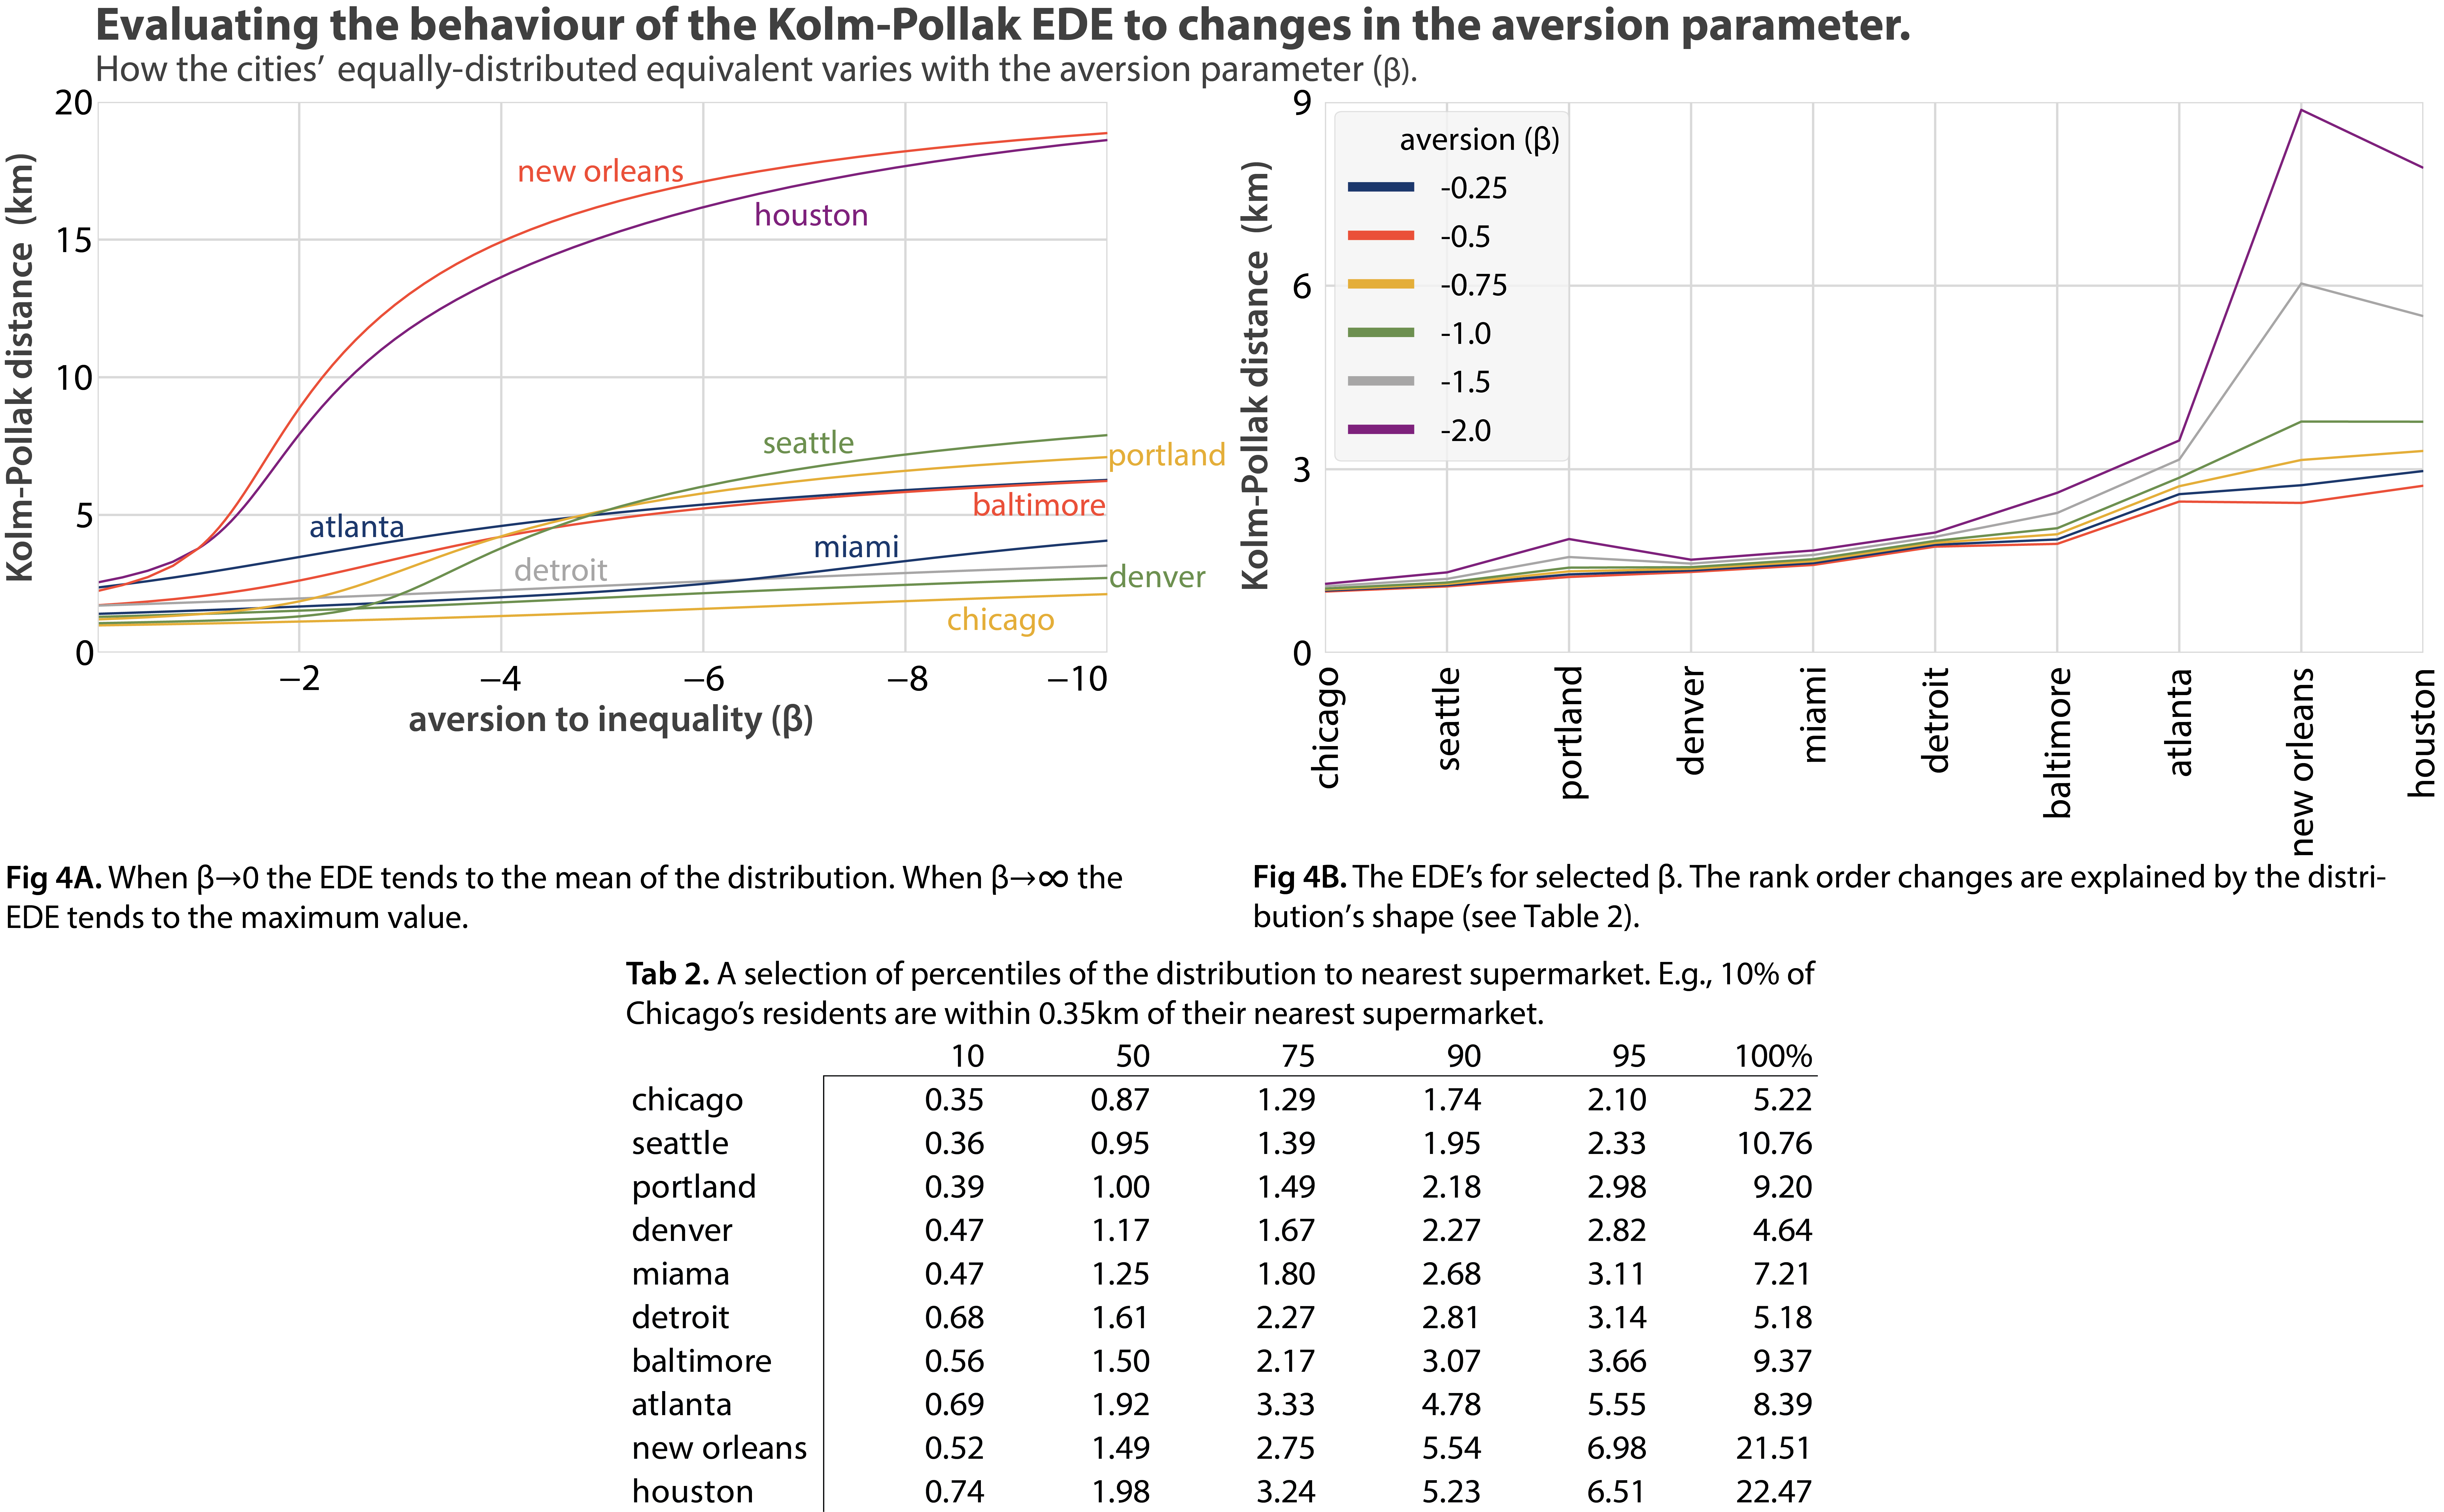
\includegraphics[width=\linewidth]{report/fig/fig3.png}
    \caption{
    Evaluating the sensitivity of the Kolm-Pollak measure and inequality to the inequality aversion parameter.
    }
    \label{fig:aversion}
\end{figure*}
\subsubsection{Grocery store access}
We see a strong level of agreement in the evaluations of the performance of the cities in providing access and equitable access to grocery stores.
These results show there is still significant challenges with grocery store access in many USA cities.
If the goal is to bring the city EDE's near or below 1.6km (1-mile), then only half of the ten evaluated are satisfactory (and this is given a low (-0.5) aversion to inequality).
Additionally, only three of these ten cities have an EDE less than 1.6km for African Americans, so there remains noticeable inequities in access to grocery stores.

New Orleans and Houston both have major challenges ahead to succeed in providing an acceptable and equitable level of access.
Some of their residents have extremely low access to grocery stores.

On the other hand, this study highlights remarkable progress in addressing the challenges of grocery store access.
Food deserts in Chicago were studied between 2007 and 2014 by \cite{Kolak2018-az}, who found major disparities in access; however, many of these disparities appear to have been addressed.
Although our study is not exactly comparable with \cite{Kolak2018-az}'s\footnote{\cite{Kolak2018-az} use a stricter definition of supermarket (for example, we include Aldi stores, which are not technically supermarkets due to their low product range)} there is nevertheless noticeable improvement.
These improvements demonstrate how awareness of access-deserts can successfully motivate action (e.g., city plans such as Chicago's \textit{Recipe for Healthy Places}).
Seattle's excellent access and equality between the demographic groups is another example of a success initiative to improve grocery store access.

Given the COVID-19 crisis we currently face, this access inequality places major health burdens on those without access to grocery stores.
People are forced to drive or take long public transit journeys to reach their nearest grocery store.
Having large stores that serve multiple communities, as opposed to having local stores, also increases the risk of transmission as it converges people from multiple communities to a common location.
This would be avoided with localized and walkable stores which would effectively create smaller, local communities.

\subsection{Disaster response: Access}
Another example of where the Kolm-Pollak EDE can be used is to evaluate or guide recovery following disasters and disruptions.
In this instance, we consider how access to grocery stores changes over time following a hurricane.
This particular example is Wilmington, North Carolina, following 2018's Hurricane Florence (using data from \cite{Logan2020-vj}).
Figure \ref{fig:florence} shows the EDE for nearest grocery store and how that recovers (similar to a resilience curve).
The EDE enables inequality considerations to be embedded into resilience and decisions on reopening stores could be guided by the impact on the EDE.
Here we show both the EDE for $\beta=-0.5$ and $\beta=-1.5$.

% \begin{figure*}[h!]
%     \centering
%     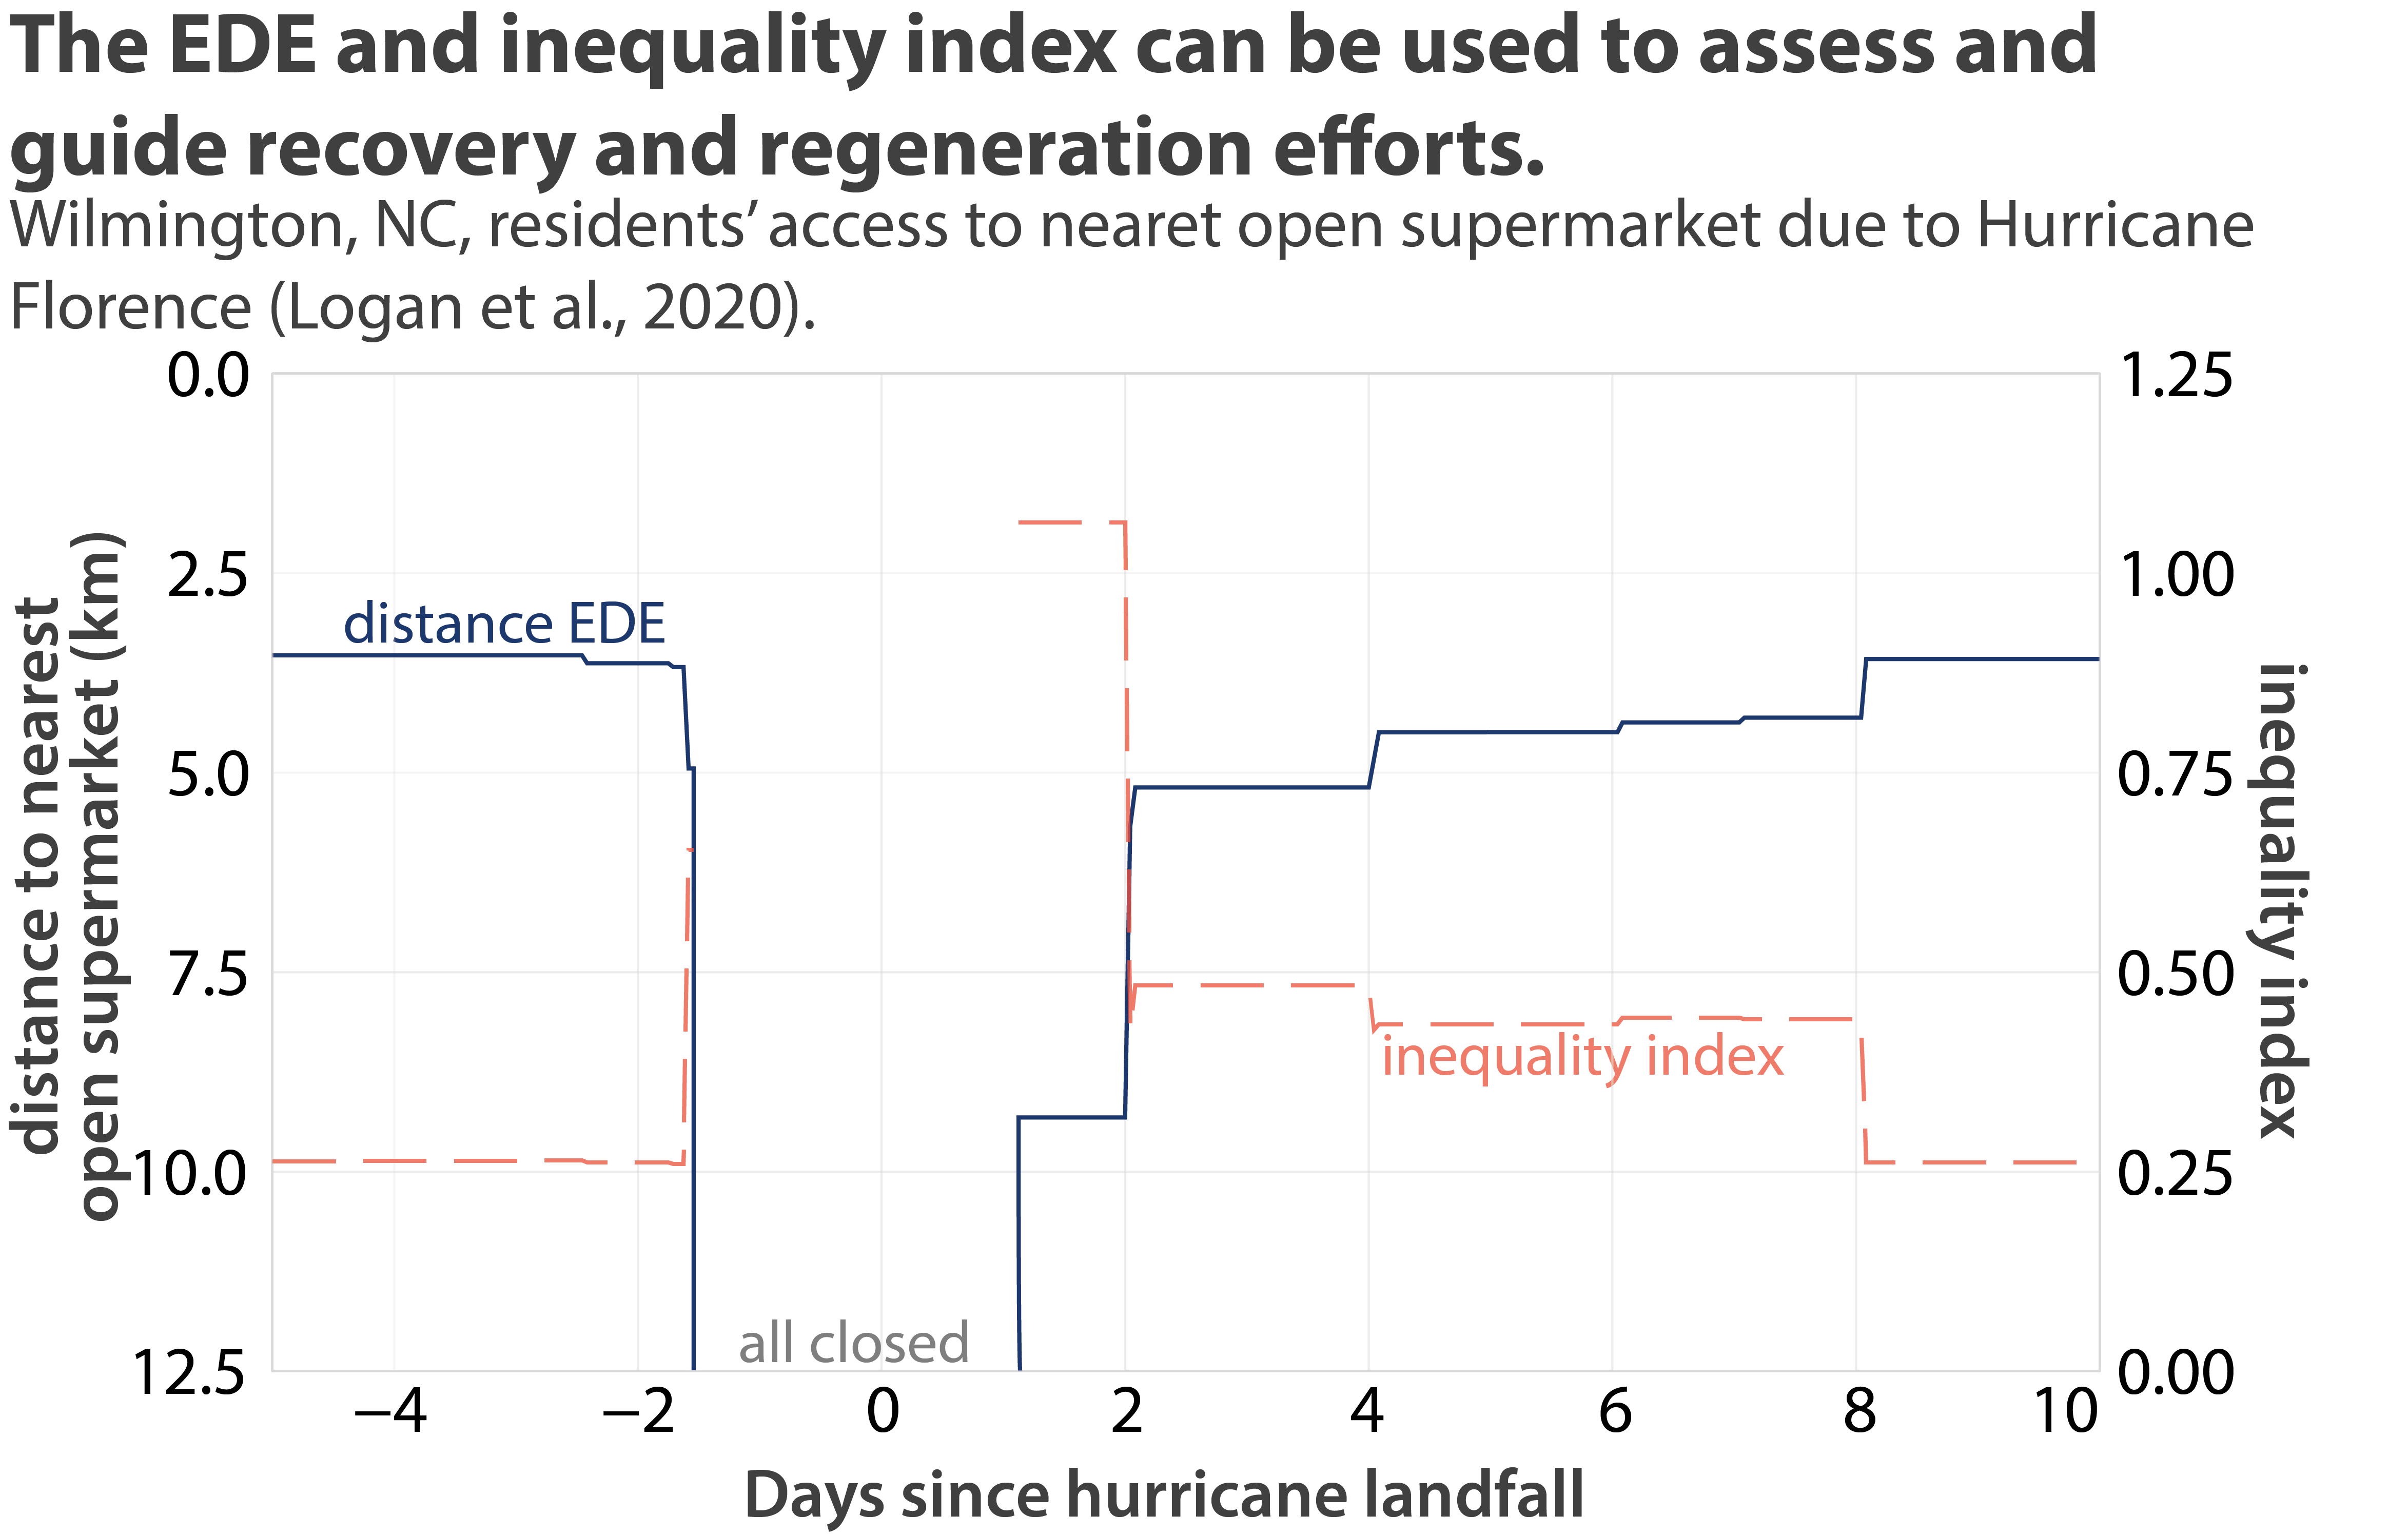
\includegraphics[width=0.5\linewidth]{report/fig/fig4.png}
%     \caption{
%     How the access to grocery stores changes over the course of a hurricane.
%     }
%     \label{fig:florence}
% \end{figure*}

\begin{figure}[!bp]
  \centering
  \begin{minipage}[b]{0.45\textwidth}
    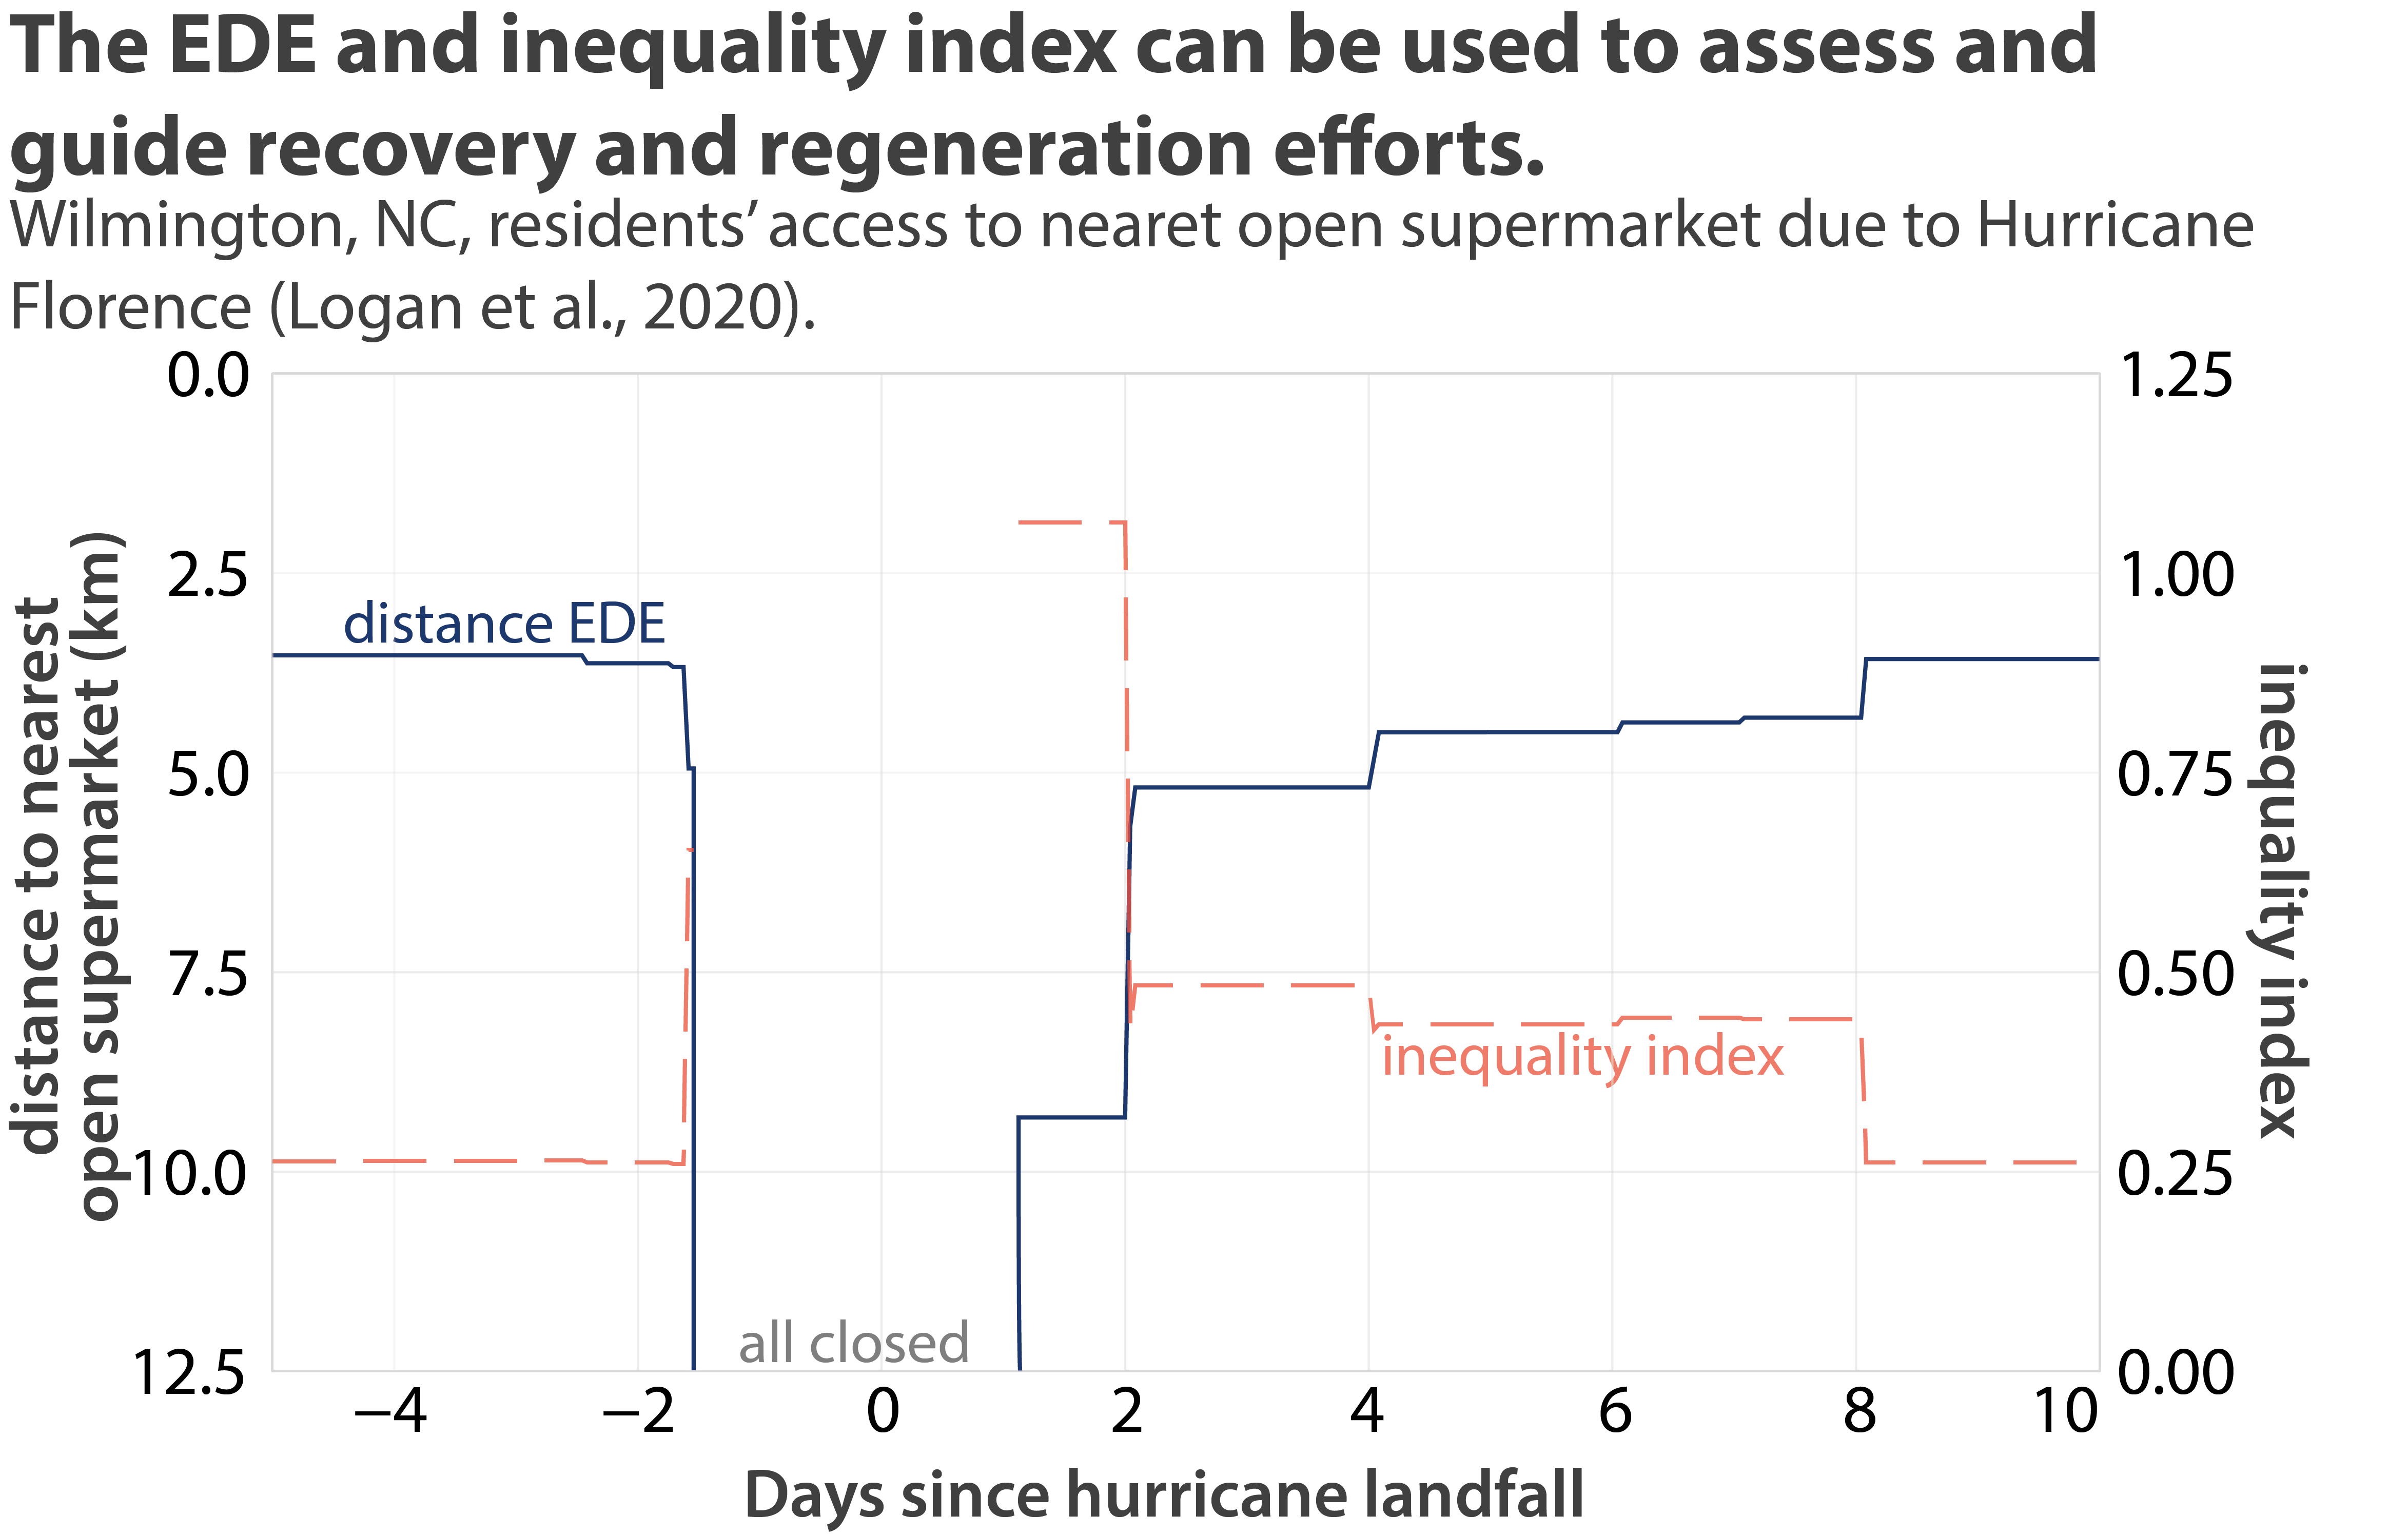
\includegraphics[width=1\linewidth]{report/fig/fig4.png}
    \caption{
    How the access to grocery stores changes over the course of a hurricane.
    }
    \label{fig:florence}
  \end{minipage}
  \hfill
  \begin{minipage}[b]{0.45\textwidth}
    \includegraphics[width=1\linewidth]{report/fig/fig5.png}
    \caption{
    Application of EDE's and inequality index beyond accessibility, but within the purview of disaster planning: impact on and recovery of electricity provision following a hurricane.
    }
    \label{fig:electricity}
  \end{minipage}
\end{figure}


\subsection{Disaster restoration: Power}
As a final example, we look at the impact on and restoration of electricity provision due to a hurricane (Figure \ref{fig:electricity}).
In this instance the quantity is not access, but rather the percentage of customers without power and the time taken to restore power per reported areal unit.
We use data from Hurricane Matthew which affected a number of states and their utility providers in 2016.
Although there are a number of factors to consider, the EDE could be used to evaluate how well utilities responded and how equitable that response was. 
For example, it is surprising that utility B has a lower percentage of customers impacted, but a noticeably higher restoration time.
Exploring the reasons and factors behind could be an independent study, we pose the question as an example of how the EDE can be used to evaluate equality within the built environment.

% \begin{figure*}[h!]
%     \centering
%     \includegraphics[width=0.5\linewidth]{report/fig/fig5.png}
%     \caption{
%     add something
%     }
%     \label{fig:electricity}
% \end{figure*}

\section{Conclusion}
The Kolm-Pollak measure provides a way of quantifying the performance and inequality of how quantities are distributed within the built environment.
This presents numerous opportunities for planners, especially with the growing interest in data-driven planning, as it enables us to evaluate the distribution of desirable and undesirable quantities and those distributions between subgroups.
While map-based visualizations are irreplaceable and will always be necessary for understanding the geographic distribution of quantities throughout a region, the EDE can be used in quantitative analysis for ranking or optimization that support decision-making, that captures inequality.
For example, where previous studies have used thresholds (e.g., ParkScore's percentage of people within 10-minute walk to nearest green space) or summary statistics in regression-type analysis, the EDE can enhance these same analysis to factor in inequality.

Practical opportunities to improve the equality of our built environment could grow following the COVID-19 crisis with the subsequent investments by governments world-wide to restart economies.
The Kolm-Pollak method enables cities to set and evaluate targets on urban characteristics, including but not limited to access to essential services. 
Policy and planning to address food-deserts and other service-deserts could foster improved, equitable access to these services which would both reduce carbon emissions and potentially improve community resilience by reducing residents' exposure to pandemics.

The Kolm-Pollak presents an opportunity for those of us working to guide decision-making in built environment contexts to reduce inequity and social injustices and ultimately enhance the  social sustainability of our communities.

\bibliography{mybibfile}

\clearpage
\newpage
\linenumbers
\appendix
%%%%%% %%%%%%%%%% %%%%%%%%%% %%%%%%%%% %%%%% SUPPLEMENTAL %%%%%%%%% %%%%%%%%%% %%%%%%%% %%%%%%%%
\section{}

\begin{table}[h]
\caption{Various metrics to evaluate a distribution and inequality indices}
\label{tab:compare_measures}
\begin{tabular}{l|RRRRRR}
\hline \hline
\multicolumn{7}{l}{\textit{Panel A. Representation of distribution (km):} $\beta=-0.5$ }\\
                                                                                   & Kolm-Pollak EDE   & Atkinson EDE   & Atkinson Adj. EDE   & Mean       & Max              &                    \\
\hline
Baltimore                                                                          & 1.85              & 0.82           & 1.89                    & 1.72       & 9.37             &                    \\
Miami                                                                              & 1.47              & 0.97           & 1.52                    & 1.41       & 7.21             &                    \\
Denver                                                                             & 1.35              & 1.02           & 1.40                    & 1.30       & 4.64             &                    \\
Detroit                                                                            & 1.77              & 0.74           & 1.80                    & 1.70       & 5.18             &                    \\
New Orleans                                                                        & 2.74              & 0.80           & 2.64                    & 2.23       & 21.51            &                    \\
Atlanta                                                                            & 2.59              & 0.63           & 2.61                    & 2.36       & 8.39             &                    \\
Portland                                                                           & 1.28              & 1.23           & 1.34                    & 1.20       & 9.20             &                    \\
Seattle                                                                            & 1.10              & 1.32           & 1.16                    & 1.07       & 10.76            &                    \\
Houston                                                                            & 2.97              & 0.62           & 2.87                    & 2.54       & 22.47            &                    \\
Chicago                                                                            & 1.02              & 1.37           & 1.07                    & 0.99       & 5.22             &                    \\

                                                                                   &                   &                &                         &            &                  &                    \\
\multicolumn{7}{l}{\textit{Panel B. Measure of inequality:} $\beta=-0.5$ }\\
                                                                                   & Kolm-Pollak Index & Atkinson Index & Atkinson Adj. Index & Gini Index & Stand. Deviation & Coef. of Variation \\
\hline
Baltimore                                                                          & 0.14              & 0.16           & 0.10                    & 0.36       & 1.18             & 0.68               \\
Miami                                                                              & 0.06              & 0.23           & 0.08                    & 0.30       & 0.82             & 0.58               \\
Denver                                                                             & 0.05              & 0.13           & 0.08                    & 0.21       & 0.74             & 0.57               \\
Detroit                                                                            & 0.06              & 0.11           & 0.06                    & 0.24       & 0.83             & 0.49               \\
New Orleans                                                                        & 0.50              & 0.22           & 0.18                    & 0.46       & 2.10             & 0.94               \\
Atlanta                                                                            & 0.23              & 0.16           & 0.11                    & 0.31       & 1.58             & 0.67               \\
Portland                                                                           & 0.08              & 0.39           & 0.12                    & 0.20       & 0.89             & 0.74               \\
Seattle                                                                            & 0.04              & 0.52           & 0.09                    & 0.32       & 0.65             & 0.61               \\
Houston                                                                            & 0.43              & 0.31           & 0.13                    & 0.26       & 1.97             & 0.78               \\
Chicago                                                                            & 0.03              & 0.17           & 0.08                    & 0.38       & 0.59             & 0.60               \\
                                                                                   & Correlation       &-0.01           & 0.88                    & 0.45       & 0.98             & 0.86               \\

\end{tabular}
\end{table}



\begin{table}[h]
\caption{Various metrics to evaluate a distribution and inequality indices}
\label{tab:compare_demographics}
\begin{tabular}{l|RRRRRR}
\hline \hline
\multicolumn{7}{l}{\textit{Panel A. Representation of distribution (km):} $\beta=-0.5$ }\\
\hline
                                                                            & Total & White & Black & Native American & Asian & Hispanic \\
Baltimore                                                                   & 1.85  & 1.67  & 1.96  & 1.82            & 1.24  & 1.70     \\
Miami                                                                       & 1.47  & 1.29  & 2.10  & 1.70            & 1.17  & 1.32     \\
Denver                                                                      & 1.35  & 1.28  & 1.66  & 1.30            & 1.38  & 1.41     \\
Detroit                                                                     & 1.77  & 1.55  & 1.82  & 1.60            & 1.35  & 1.40     \\
New Orleans                                                                & 2.74  & 2.04  & 3.13  & 2.14            & 2.57  & 2.03     \\
Atlanta                                                                     & 2.59  & 1.76  & 3.20  & 2.46            & 1.54  & 2.25     \\
Portland                                                                    & 1.28  & 1.27  & 1.22  & 1.29            & 1.46  & 1.24     \\
Chicago                                                                     & 1.02  & 0.88  & 1.29  & 0.91            & 0.77  & 0.92     \\
Seattle                                                                     & 1.10  & 1.10  & 1.10  & 1.05            & 1.11  & 1.10     \\
Houston                                                                     & 2.97  & 2.62  & 3.93  & 2.95            & 2.14  & 2.93     \\
\\
\multicolumn{7}{l}{\textit{Panel B. Measure of inequality:} $\beta=-0.5$ }\\
\hline
                                                                            & Total & White & Black & Native American & Asian & Hispanic \\
Baltimore                                                                   & 0.14  & 0.17  & 0.11  & 0.18            & 0.10  & 0.20     \\
Miami                                                                       & 0.06  & 0.04  & 0.08  & 0.07            & 0.05  & 0.04     \\
Denver                                                                      & 0.05  & 0.04  & 0.07  & 0.05            & 0.05  & 0.06     \\
Detroit                                                                     & 0.06  & 0.06  & 0.06  & 0.06            & 0.02  & 0.07     \\
New Orleans                                                                & 0.50  & 0.50  & 0.49  & 0.32            & 0.41  & 0.32     \\
Atlanta                                                                     & 0.23  & 0.10  & 0.26  & 0.24            & 0.08  & 0.21     \\
Portland                                                                    & 0.08  & 0.08  & 0.05  & 0.11            & 0.11  & 0.05     \\
Chicago                                                                     & 0.03  & 0.02  & 0.04  & 0.02            & 0.02  & 0.02     \\
Seattle                                                                     & 0.04  & 0.04  & 0.03  & 0.04            & 0.04  & 0.04     \\
Houston                                                                     & 0.43  & 0.37  & 0.56  & 0.38            & 0.17  & 0.37    
\end{tabular}
\end{table}


\clearpage
\newpage
\section{Code}
\label{appendix:code}

This is an extract of the code provided in the GitHub repository: []

\begin{lstlisting}[language=Python]
"""
Inputs:
    a = distribution of data, type=list
    weight (optional) = list of len(a)
    kappa (optional) = int < 0
    beta (optional, default = -0.5)
        if the distribution is of an undesirable (e.g., exposure)
            beta = int < 0 
        if it is a desirable property (e.g., income) 
            beta = int > 0 
    epsilon (optional, default = 0.5) = int > 0
Output:
    Kolm-Pollak EDE & Index (kappa)
    Atkinson Adjusted EDE & Index (beta)
    Atkinson EDE & Index (epsilon)
    Gini Index
"""

import numpy as np
from scipy.integrate import simps

def kolm_pollak_ede(a, beta = None, kappa = None, weight = None):
    """returns the Kolm-Pollak EDE"""
    a = np.asanyarray(a)

    if kappa is None:
        if beta is None:
            raise TypeError("you must provide either a beta or kappa aversion parameter")
        kappa = calc_kappa(a, beta, weight)

    if weight is None:
        ede_sum = np.exp(a*-kappa).sum()
        N = len(a)
    else:
        ede_sum = np.multiply(np.exp(a*-kappa), weight).sum()
        N = sum(weight) # for a weighted average

    ede = (-1 / kappa) * np.log(ede_sum / N)
    return(ede)


def kolm_pollak_index(a, beta = -0.5, kappa = None, weight = None):
    """returns the Kolm-Pollak Inequality Index"""
    if weight is None:
        x_mean = np.mean(a)
    else:
        x_mean = np.average(a, weights = weight)

    a = a - x_mean

    inequality_index = kolm_pollak_ede(a, beta = beta, kappa = kappa, weight = weight)

    return(inequality_index)

\end{lstlisting}

\end{document}

